% ============================================================
% 4. METHOD: DIAL
% ============================================================
\begin{figure*}[t]
	\centering
	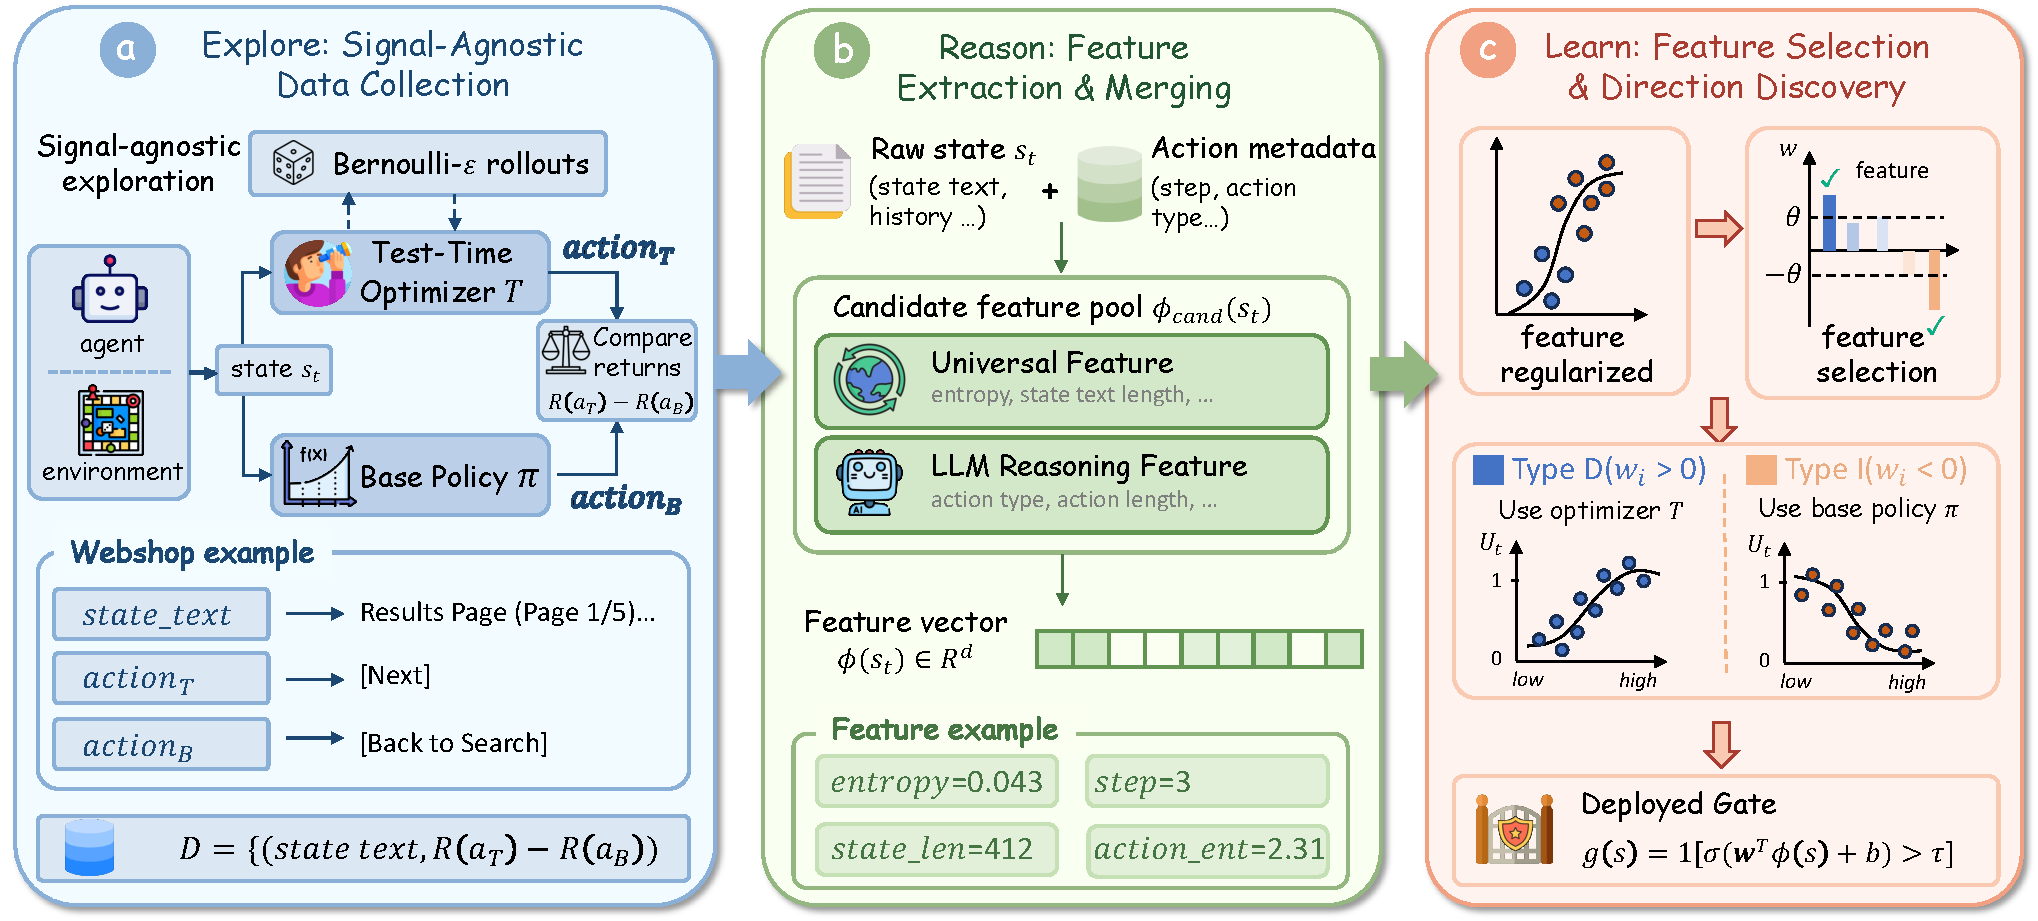
\includegraphics[width=\textwidth]{figures/dial_pipeline4.pdf} 
    \vspace{-0.2in}
	\caption{\textbf{The DIAL pipeline.}
		\textbf{(a) Explore}: collect signal-agnostic $(s, U)$ pairs via Bernoulli-$\varepsilon$ rollouts.
		\textbf{(b) Reason}: build a candidate feature pool $\phi(s)$ from universal metrics combined with LLM-proposed task-specific features.
		\textbf{(c) Learn}: fit an $\ell_1$-regularized logistic gate, whose signed weights jointly perform feature selection and recover per-environment direction (Type~D: $w_i{>}0$; Type~I: $w_i{<}0$).}
	\label{fig:method_overview}
\end{figure*}
\vspace{-0.1in}
\section{Direction-Informed Adaptive Learning}
\label{sec:method}
\vspace{-0.1in}
DIAL reframes gating from difficulty estimation to intervention-utility estimation: it trains on counterfactual optimizer utility rather than difficulty or correctness proxies, and uses signal-agnostic exploration so that the learned gate can discover when each feature indicates positive or negative rollout value instead of inheriting a fixed direction from the data collection rule.
The analysis in \S\ref{sec:signal-landscape} implies three constraints for any cross-setting adaptive gate. It must (i) \emph{discover} the signal-utility direction per (environment, backbone) pair rather than hardcoding it; (ii) draw from a \emph{multi-signal feature pool} that approximates the latent state type $\tau(s)$, since no single signal is reliable across settings; and (iii) collect training data \emph{without conditioning on} the very signal whose direction is unknown, otherwise the data is biased toward the prior assumption. DIAL satisfies these three constraints in three stages (Fig.~\ref{fig:method_overview}): randomized exploration (\S\ref{sec:explore}), feature construction (\S\ref{sec:reason}), and sparse gate fitting (\S\ref{sec:learn}).

\vspace{-0.1in}
\subsection{Explore: Signal-Agnostic Data Collection}
\label{sec:explore}
\vspace{-0.05in}
The exploration stage collects the $(s, U)$ pairs used to fit the gate, under one central constraint: the collection policy must remain independent of any signal whose semantics we are trying to learn. A gate trained on uncertainty-triggered states would systematically under-sample the states that determine $\rho$'s sign, baking the prior assumption into the training data instead of testing it.

DIAL therefore uses the simplest policy consistent with this constraint. At each step~$t$ in episode~$i$, a uniform random coin flip with probability $\varepsilon_{\text{explore}}$ determines whether to trigger the optimizer~$T$ ($z_t^{(i)}{=}1$) or use the base action ($z_t^{(i)}{=}0$). For each step with $z_t^{(i)}{=}1$, we estimate utility by paired counterfactual rollouts from the same state snapshot: we fork the environment, execute both the optimizer's chosen action and the base action via truncated rollouts of horizon $H$, and record which yields a higher return. We set $U_t^{(i)} = 1$ if the optimizer's action wins, and $0$ otherwise. The Bernoulli trigger eliminates selection bias, and the paired design eliminates baseline bias; the remaining approximation is the truncation horizon $H$. Aggregating across $N_{\text{explore}}$ episodes yields the dataset:
\begin{equation}
  \mathcal{D} = \bigl\{
    \bigl(\phi(s_t^{(i)}),\; U_t^{(i)}\bigr)
    : z_t^{(i)} = 1
  \bigr\}_{t, i},
  \label{eq:dataset}
\end{equation}
where $\phi(s)$ is the feature vector. Per-environment estimation details are in Appendix~\ref{app:environment}.

\vspace{-0.1in}
\subsection{Reason: Feature Construction}
\label{sec:reason}
\vspace{-0.05in}
The next stage builds the candidate feature pool $\phi_{\text{cand}}(s)$. This pool must be rich enough to capture each environment's informative signals, but not so environment-specific that deployment requires manual engineering per task.

DIAL's candidate pool combines two layers. The first is a small set of universal features defined identically across environments: \texttt{step\_count}, \texttt{token\_entropy}, \texttt{evidence\_count}, \texttt{num\_available\_actions}, and \texttt{is\_finish} (definitions in Table~\ref{tab:universal-features}). Signals an environment does not naturally expose (e.g., \texttt{evidence\_count} outside QA-style tasks) default to zero, requiring no per-environment engineering. The second is an LLM-generated layer: an LLM receives a summary of $\mathcal{D}$ and proposes task-specific feature hypotheses $\phi_{\text{LLM}}(s)$, forming $\phi_{\text{cand}}(s) = \phi_{\text{univ}}(s) \cup \phi_{\text{LLM}}(s)$. The $\ell_1$ penalty in the next stage automatically discards uninformative proposals, so the LLM layer can propose freely without degrading gate quality. We show in \S\ref{sec:ablation} that the universal pool alone already outperforms all fixed-direction baselines, and the LLM layer adds further gains in environments where universal features are inadequate. We provide the prompt template and per-environment ablation in Appendix~\ref{app:llm-feature-layer} and Appendix~\ref{app:llm-features}.

\vspace{-0.1in}
\subsection{Learn: Sparse Linear Gate}
\label{sec:learn}
\vspace{-0.05in}

Given $\mathcal{D}$ and $\phi_{\text{cand}}$, DIAL fits an $\ell_1$-regularized logistic regression with the binary cross-entropy loss, where the regularization strength $\lambda$ controls sparsity over $\phi_{\text{cand}}$ so that uninformative features drop out. Let $(\mathbf{w}^*, b^*)$ denote the fitted weights and bias. The deployed gate is
\begin{equation}
  g(s) = \mathbf{1}\!\left[\mathrm{sigmoid}(\mathbf{w}^{*\top} \phi(s) + b^*) > \tau\right],
  \label{eq:gate}
\end{equation}
with threshold $\tau$ set by cross-validation on $\mathcal{D}$. At deployment, the gate requires only a feature evaluation and a single sigmoid: no extra LLM calls, no $K$-way voting, no calibration query. This zero-overhead deployment contrasts with prior gating methods that incur per-step costs (e.g., CATTS triggers $K{=}5$ forward passes per step, AUQ issues a confidence query every step).

\textbf{Signed weights as a diagnostic.}
The $\ell_1$ penalty simultaneously performs feature selection and direction discovery. The sign of each fitted weight provides an interpretable per-environment estimate of how the feature relates to optimizer utility: $w_i > 0$ indicates that feature~$i$ behaves as a decision-difficulty proxy in this setting, where larger values increase expected rollout value; $w_i < 0$ indicates an intervention-unsuitability proxy, where larger values mark states in which rollouts are less likely to help; and $w_i \approx 0$ indicates that the feature is uninformative. The complete pipeline, including online adaptation for drifting environments and detailed cost accounting, is in Appendix~\ref{app:dial-details}.